%
%  untitled
%
%  Created by Asger Pedersen on 2012-01-04.
%  Copyright (c) 2012 . All rights reserved.
%
\documentclass[]{article}

% Use utf-8 encoding for foreign characters
\usepackage[utf8]{inputenc}

% Setup for fullpage use
\usepackage{fullpage}

\usepackage{hyperref}
\usepackage{pdfpages}
% Uncomment some of the following if you use the features
%
% Running Headers and footers
%\usepackage{fancyhdr}

% Multipart figures
%\usepackage{subfigure}

% More symbols
%\usepackage{amsmath}
\usepackage{amssymb}
%\usepackage{latexsym}

% Surround parts of graphics with box
\usepackage{boxedminipage}

% Package for including code in the document
\usepackage{listings}

% If you want to generate a toc for each chapter (use with book)
\usepackage{minitoc}

% This is now the recommended way for checking for PDFLaTeX:
\usepackage{ifpdf}

%\newif\ifpdf
%\ifx\pdfoutput\undefined
%\pdffalse % we are not running PDFLaTeX
%\else
%\pdfoutput=1 % we are running PDFLaTeX
%\pdftrue
%\fi

\usepackage{ifpdf}
\title{ Project Course: Development Studio \\ Deliverable 4: Sprint \#3}
\author{ Asger Pedersen, Kristoffer Cobley, Hari Charan \& Jesper Tved }
\setlength{\parindent}{0pt}
\setlength{\parskip}{2ex}
\linespread{1.3}

\begin{document}

\ifpdf
\DeclareGraphicsExtensions{.pdf, .jpg, .tif}
\else
\DeclareGraphicsExtensions{.eps, .jpg}
\fi

\maketitle
\setcounter{tocdepth}{1}
\tableofcontents
\newpage
\section{Sprint Material} % (fold)
\label{sec:Sprint Material}
\subsection{Version} % (fold)
\label{sub:Version}
The current state of our app has version 0.0.1. Meaning that the app is still alpha quality, with some functionality implementet, but lot of unfinished work.
% subsection Version (end)
\subsection{Source code} % (fold)
\label{sub:Source code}
We still use Git and GitHub. The source code is available at: \verb!https://github.com/mundane/ETA_analytics!, in the app folder. The other folders contains prototypes and experiments.
% subsection Source code (end)
\subsection{Sprint Explanation}
The burndown chart shows that, in spite of exams and easter holidays stalled the progress of development in the beginning of the sprint, we did manage to finish some of the tasks within the sprint time frame.
\begin{figure}[h!]
  \centering
    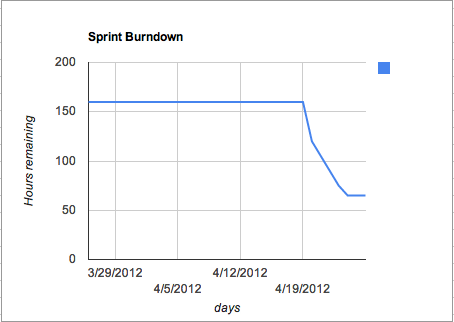
\includegraphics[width=0.8\textwidth]{images/burndown.png}
	\caption{Burndown chart for sprint \# 2. Easter holidays and exams is the reason for the steep curve.}
\end{figure}

\subsection{User Stories}
For sprint \# 2 we had the following user stories: \\
As an analytic \\
I want to make pie charts, column charts, bar charts, etc \\
So that I can make data more presentable \\

As an analytic \\
I want to make charts interactive  \\
So that I can make data more presentable \\

As an analytic \\
I want a way to show selected data from the chart \\
So that I can make data more presentable\\

As an analytic \\
I want to save data for later sessions \\
So I can continue working on datasets \\

\subsection{Tasks} % (fold)
\label{sub:Tasks}
We divided the stories up in the following tasks
% subsection Tasks (end)Tasks
\begin{itemize}
	\item Read up on the MVC model
	\item Research testing tools for Sencha
	\item Research JSLint
	\item Convert CSV format to JSON
	\item Create datagrid from JSON
	\item Make integration to Jstat in the datagrid view
	\item Create charts
\end{itemize}










% section Sprint Material (end)


\section{Sprint Retrospective} % (fold)
\label{sec:Sprint Retrospective}

% section Sprint Retrospective (end)

\section{Learning Goals} % (fold)
\label{sec:Learning Goals}

% section Learning Goals (end)
\section{Architectural Description} % (fold)
\label{sec:Architectural Description}

In the following we will be describing the current software architecture for our system. An architectural description could be used as a basis for stakeholder communication, as part of an on-going software design process or to evaluate different architectures \cite{christensen}. In the following we will be using the recommendations found in \cite{christensen} to describe the software architecture. In particular we will be using different viewpoints to communicate the overall structure of the system. In the following we will be looking at the model, C\&C view respectively, we will not be looking at the deployment view in our case, as our system is simple enough that this view would not add much to an overview.

\subsection{Model View}



\subsection{C\&C View}


% section Architectural Description (end)
\section{Documentation} % (fold)
\label{sec:Documentation}
Chosing to build our application in JavaScript means that finding a documenting tool was not particular easy, as tools like JavaDoc and doxygen are not applicable to JavaScript. In our research we happened upon JSdoc, \url{http://code.google.com/p/jsdoc-toolkit}
% section Entity Documentation (end)
\section{Anomalies} % (fold)
\label{sec:Anomalies}

\subsection{Code Inspection} % (fold)
\label{sub:Code Inspection}



CodeCode Inspection workshop involved us, presenting project source code to an inspection team,
who upon reviewing, complied a set of suggestions and best practices.

Since the feedback from the review team was low and not comprehensive, further addition inhouse inspection was conducted on possible 
code refactoring and possible rework.

The comments received are presented below:

Comments on Source code: ``The source code has to be commented and appropriate description fucntionalities should be added''.

Consider JavaScript Compressor: ``As rich applications is built with larger JavaScript code bases, the need for JavaScript compression 
to keep bandwidth and page load times as small as possible is becoming more important for faster load times and more enjoyable user experiences''.

Consider Jquery:Think of using jQuery(might speed up things/less code: jQuery is a cross-browser JavaScript library designed to simplify the client-side scripting of HTML
 
Consider Jslint: is a web-app which takes a JavaScript source and scans it. If it finds a problem, it returns a message describing the problem and an approximate solution. 

% subsection Code Inspection (end)
\subsection{Rework and Code Refactoring} % (fold)
\label{sub:rework}

% subsection subsection name (end)

Code Documentation guide:Comments on our source codes and fucntionalities description has been added using Docco, see section \ref{sec:Documentation}

JavaScript Compressor: A statergy to make use of a JavaScript optimizer later in the project finsihing stages has been decided.
Closure Compiler- a google service for java code optimizer will be used for this purpose.Instead of compiling from a source language to machine code, it compiles from JavaScript to better JavaScript. It parses your JavaScript, analyzes it, removes dead code and rewrites and minimizes what's left. 
It also checks syntax, variable references, and types, and warns about common JavaScript pitfalls. 

Jquery: We have decided not to use Jquery instead of Sencha because, Sencha is far more extensive than its competitors, with a vast array of UI    
components, explicit iOS and Android support, storage and data binding facilities using JSON and HTML5 offline storage, and more.

For all that apparent extra weight and bulky library, Sencha performed better and was more reliable.

% section Anomalies (end)
\appendix
\section{Scrum Material} % (fold)
\label{sec:Scrum Material}

% section Scrum Material (end)
%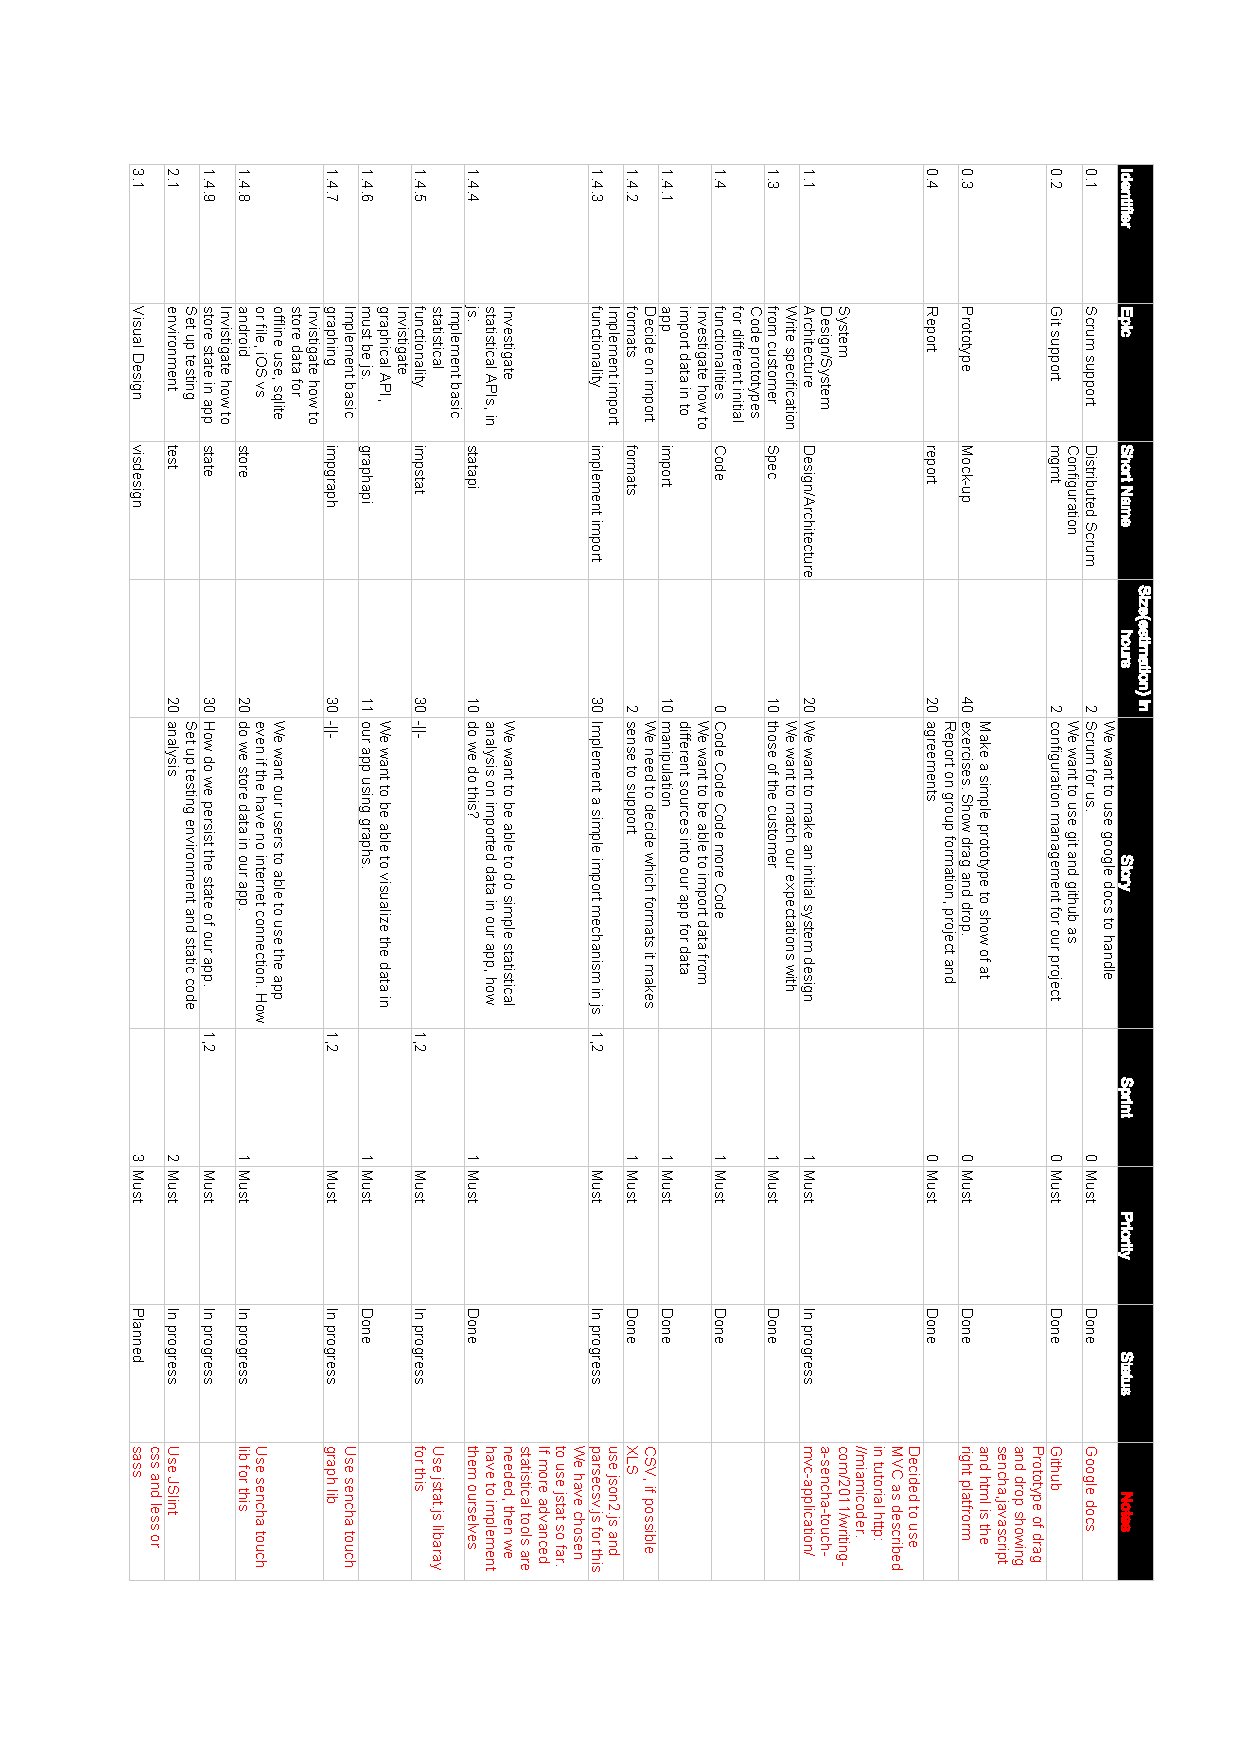
\includepdf[pages={-}]{images/backlog1.pdf}
%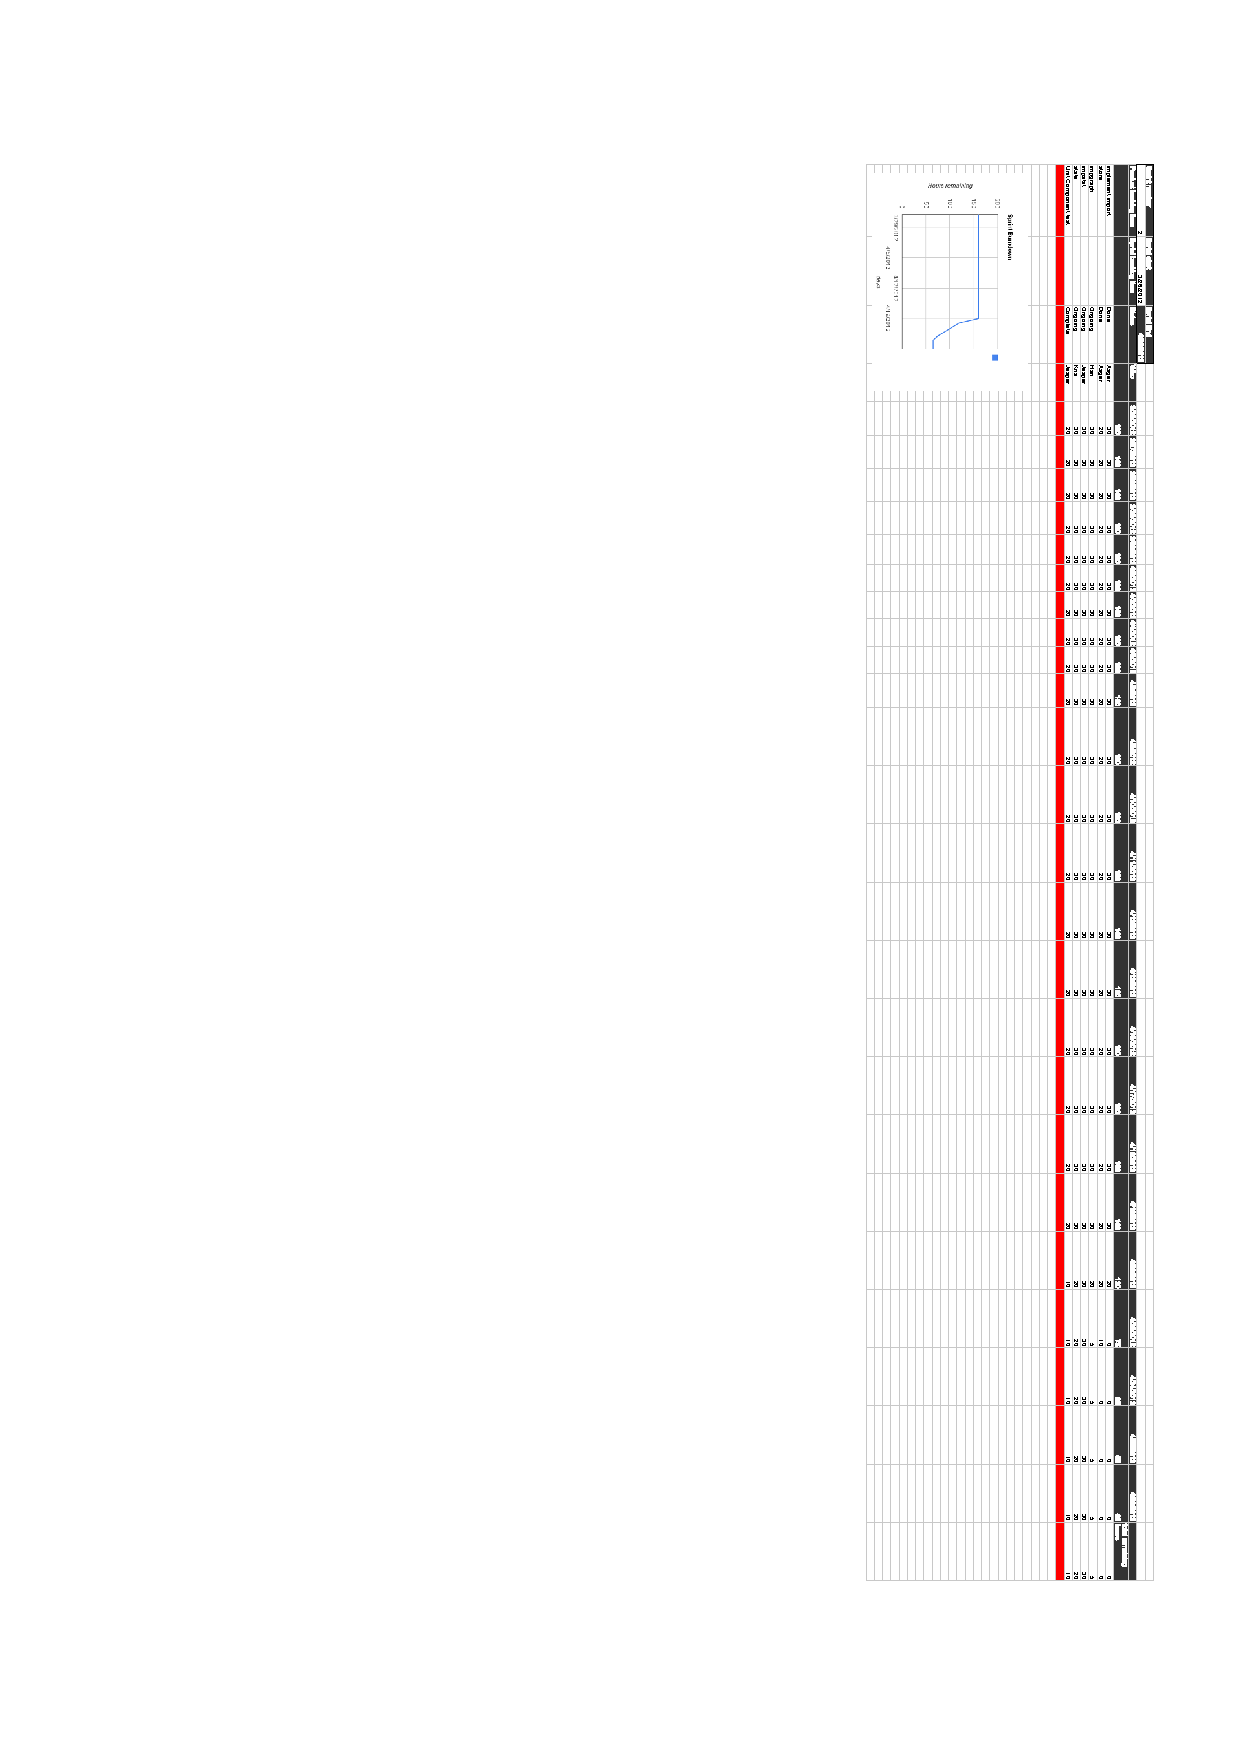
\includepdf[pages={-}]{images/sprint1.pdf}

\bibliographystyle{plain}
\bibliography{}
\end{document}